%!TEX root = ../DevaramaniS-[RnD-MT]Report.tex

\chapter{Experimental Evaluation and Results}\label{chap:experiment}

The following chapter presents the \textit{proof of concept} and evaluation of the proposed extension to \textit{Popov-Vereshchagin solver}. All the experiments are conducted in a simulation environment. The obtained results are analyzed based on the physical behavior of the system. 


\section{Experimental Setup}
This section describes the overall experimental setup designed to test the proposed extension to the solver for MPO-700 robot base. The modeled tree structure of MPO-700 base is tested for its behavior by providing external forces and feed-forward torques.  The other input parameters ($q$, $\dot{q}$, ($\ddot{q}$), $A_N$ and $b_N$) are kept constant. The computed joint and base accelerations are interpreted based on the magnitudes and directions, and are analyzed with respect to the physical behavior of the system. Further, the test cases presented is based on two wheel configurations. The results are analyzed based on the configuration.  


\paragraph{}The following experiments are based on some of the assumptions, they are,

\begin{enumerate}
	\item The wheel and joint configuration is assumed to be the same in all experiments.  
	\item The convention used to represent joint and base motions follow \textit{right-hand rule}.
	\item The friction between joints or at the point of contact of wheel and ground is not considered in experiments.
	\item The virtual rolling constraint is not modeled in the kinematic chain and hence not considered in test cases.
	\item The units of physical quantities are not considered by the solver, however, all the quantities in experiments are assumed to be consistent with each other.
	\item The rigid offset between orientation and drive joints, introduce a constraint on wheel's rotation about \textit{z-axis}. This is a natural constraint imposed by the model and hence not defined explicitly in constraint matrix.
	\item The experimental results are evaluated with respect to the physical behavior of system. However, there are some factors such as friction, virtual rolling constraints are not considered. Because, the these factors are not modeled currently by the solver.
\end{enumerate}

Following are the input and output parameters described briefly. The input parameters that are kept constant throughout the experiment are,

\begin{itemize}
	\item \textit{Input joint angles (q), velocities ($\dot{q}$) and accelerations ($\ddot{q}$)} = 0 for all joints
	\item \textit{Linear constraint matrix ($A_N$):} This defines the directions of the acceleration constraints on the end-effectors (wheels). In our case, the wheels are constrained along \textit{linear-y} (sliding constraint), \textit{linear-z} (no acceleration perpendicular to the ground) and \textit{angular-x} (wheel should not ``roll'' about x-axis). The $A_N$ matrix described for all the wheels is given by, 
	\begin{equation}
		A_N = \begin{pmatrix}
		 0 & 0 & 1 \\
		 0 & 0 & 0 \\
		 0 & 0 & 0 \\
		 0 & 0 & 0 \\
		 1 & 0 & 0 \\
		 0 & 1 & 0 \\
		\end{pmatrix}
	\end{equation} 
	\item \textit{Beta vector ($b_N$):} This defines the acceleration energy vector corresponding to directions of applied constraints. Since the wheels are constrained to not to have acceleration along linear-y, linear-z and angular-z, the $b_N$ vector for each wheels is given by,
	\begin{equation}
		b_N = \begin{pmatrix}
		0 \\
		0 \\
		0
		\end{pmatrix}
	\end{equation}
\end{itemize}

As mentioned earlier, the task specification for the experiments includes external force ($F_{ext}$) and feed-forward torques ($\tau$) applied to the system. The external force is a six-dimensional vector expressed in Cartesian space, and it is applied at the robot base. According to the KDL conventions, $F_{ext}$ is represented as, 
\begin{equation}
	F_{ext} = \begin{pmatrix}
		f_x \\
		f_y \\
		f_z\\
		\tau_x \\
		\tau_y \\
		\tau_z\\
	\end{pmatrix}
\end{equation} 

where, the first three entries corresponds to linear forces and last three parameters are angular torques. The feed-forward torques are applied to each of the joints. Initially, these values are set to zero. To simplify the representation of the joints, letter ``o'' is used to denote orientation (caster) joints and ``d'' is used to denote drive joints (refer to figure \ref{fig:conventions} for joint assignments). 

Furthermore, the solver outputs that are analyzed in the experiment are - $\ddot{q}$ and $\ddot{X}$. 
\begin{itemize}
	\item \textit{Joint accelerations ($\ddot{q}$):} Represents the resultant accelerations at every joints. In the table below, the order of all the joint acceleration are, o = [o1, o2, o3, o4] and d = [d1, d2, d3, d4]. 
	\item \textit{Base acceleration:} Describes the Cartesian acceleration of the mobile base.
\end{itemize} 

The table \ref{tab:experiment} displays the wheel configurations, task specification (joint torques, external forces) and solver results (base and joint accelerations). Further, each of the cases and its results are analyzed. 
\begin{table}[h!]
	\renewcommand{\arraystretch}{2.3}
	\centering
	\resizebox{\textwidth}{8.2cm}{%
		\begin{tabular}{|M{5cm}|M{2cm}|M{2.5cm}|M{7.5cm}|}
			\hline
			{\textbf{\textit{Wheel Configuration}}} & \textbf{\textit{Task specification}} & \multicolumn{2}{M{8cm}|}{\textbf{\textit{Solver Output}}} \\ \cline{3-4} & & \textbf{\textit{Base acceleration}} & \textbf{\textit{Joint acceleration}} \\ \hline
			\multirow{5}{*}{ \begin{minipage}{.3\textwidth}
					Wheel configuration 1
					\begin{center}
						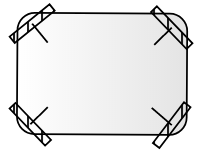
\includegraphics[scale=0.55]{images/w1.png}
					\end{center}
				\end{minipage} } & $\tau_z$ = 10 &  $\dot{\omega}_z$ = 1.5619 & \begin{minipage}{.48\textwidth}
				\centering
				o = $[0.1735, -3.2973, -3.2973, 0.1735]$ \\
				
				d = $[0.00048 ,0.00048, 0.00048, 0.00048]$
			\end{minipage} \\ \cline{2-4}
			& $f_x = 50$ & $\dot{v}_x = 0.19112$ & \begin{minipage}{.48\textwidth}
				\centering
				o = $[4.24732, 4.24732, 4.24732, 4.24732]$ \\
				
				d = $[0.00119 ,0.00119, 0.00119, 0.00119]$
			\end{minipage} \\ \cline{2-4} 
			& \begin{minipage}{.15\textwidth}
				\centering
				$\tau_{d1} = 1$ \\
				$\tau_{d2} = 1$ \\
				$\tau_{d3} = 1$ \\
				$\tau_{d4} = 1$
			\end{minipage} & Zero & \begin{minipage}{.48\textwidth}
			\centering
			o = $[0.00209, 0.00210, 0.00210, 0.00209]$ \\
			
			d = $[65.711 ,65.711, 65.711, 65.711]$
		\end{minipage}  \\ \cline{2-4} 
		& $\tau_x$ = 20 &  Zero & \begin{minipage}{.48\textwidth}
			\centering
			o = $[0.0, 0.0, 0.0, 0.0]$ \\
			
			d = $[0.0, 0.0, 0.0, 0.0]$
		\end{minipage} \\ \cline{2-4}
		& $f_z$ = 5 &  Zero & \begin{minipage}{.48\textwidth}
			\centering
			o = $[0.0, 0.0, 0.0, 0.0]$ \\
			
			d = $[0.0, 0.0, 0.0, 0.0]$
		\end{minipage} \\ \hline
		
		\multirow{6}{*} {\begin{minipage}{.26\textwidth}
				Wheel configuration 2
				\begin{center}
					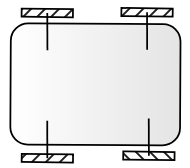
\includegraphics[scale=0.55]{images/w2.png}
				\end{center}
			\end{minipage}} & $\tau_z$ = 10 &  $\dot{\omega}_z$ = 0.49322 & \begin{minipage}{.48\textwidth}
			\centering
			o = $[3.2268, -4.2133, -4.2133, 3.2268]$ \\
			
			d = $[0.00104 ,0.00104, 0.00104, 0.00104]$
		\end{minipage}  \\ \cline{2-4}
		& $f_x = 50$ & $\dot{v}_x = 0.35370$ & \begin{minipage}{.48\textwidth}
			\centering
			o = $[0.0, 0.0, 0.0, 0.0]$ \\
			
			d = $[0.0, 0.0, 0.0, 0.0]$
		\end{minipage} \\ \cline{2-4}
		& \begin{minipage}{.15\textwidth}
			\centering
			$\tau_{d1} = 1$ \\
			$\tau_{d2} = 1$ \\
			$\tau_{d3} = 1$ \\
			$\tau_{d4} = 1$
		\end{minipage} & Zero & \begin{minipage}{.48\textwidth}
		\centering
		o = $[0.0, 0.0, 0.0, 0.0]$ \\
		
		d = $[65.711 ,65.711, 65.711, 65.711]$
	\end{minipage} \\ \cline{2-4}
	& $\tau_x$ = 20 &  Zero & \begin{minipage}{.48\textwidth}
		\centering
		o = $[0.0, 0.0, 0.0, 0.0]$ \\
		
		d = $[0.0, 0.0, 0.0, 0.0]$
	\end{minipage} \\ \cline{2-4}
	& $f_y$ = 10 &  $\dot{v}_y = 0.0259$ & \begin{minipage}{.48\textwidth} 
		\centering
		o = $[0.8155, -0.8155, 0.8155, -0.8155]$ \\
		
		d = $[0.0002,-0.0002,0.0002,-0.0002]$
	\end{minipage} \\ \cline{2-4}
	& $f_z$ = 5 &  Zero & \begin{minipage}{.4\textwidth}
		\centering
		o = $[0.0, 0.0, 0.0, 0.0]$ \\
		
		d = $[0.0, 0.0, 0.0, 0.0]$
	\end{minipage} \\ \hline
	
\end{tabular}}\renewcommand{\arraystretch}{3}
\caption{Experimental analysis}
\label{tab:experiment}
\end{table}

\section{Motion estimation}
Given the task specification, the robot motion is interpreted based on the obtained base and joint accelerations. The experiments also test for the resultant acceleration when task specification (external force and feed-forward torques) conflicts defined constraints. For these cases, it is expected to have zero acceleration both at joints and base.
%For the first wheel configuration, each of the test cases are described below,
\subsubsection*{Wheel configuration 1}
The orientation and drive wheels are oriented $45^0$ with respect to the default configuration (in table \ref{tab:experiment}). 

\subsubsection*{Case 1}
\hspace{20pt}An external torque of 10 units is applied at the base. Physically, the base is expected to rotate in the direction of applied torque (positive). However, the caster joints rotate in opposite direction with respect to the base. This behavior is due to the inertia of the wheel, which introduces a delay in rotation and generates a reaction force. In the physical system, the friction at the contact point and virtual sliding and rolling constraints also contributes to this reaction force. However, the solver only models sliding constraints and do not explicitly model the friction. Based on this interpretation, the orientation joints are expected to rotate in negative direction. But the solver results are inconsistent, where two of the caster joints (o1 and o4) are positive and other two joints (o2 and o3) are negative. Additionally, in terms of magnitude, the drive joints are expected to have higher acceleration than caster. This behavior is not reciprocated by the obtained results. 

%Nevertheless, the drive joints are expected to accelerate in the direction of base rotation. Therefore, the drive joint acceleration are expected to be negative (based on right-hand rule). 

Although, the caster joints introduces a delay and rotates opposite direction with respect to the base, the drive wheels are expected to accelerate (rotate about \textit{y-axis}) in the direction of base rotation. Referring to the frame assignments in figure \ref{fig:tree-MPO}, the angular acceleration of drive wheels result in negative values. But the solver results are positive.  

\paragraph{}Considering the base acceleration, when a positive torque of 10 units is applied to a robot base, it is expected to have a positive angular acceleration. This reasoning do not completely apply for all system (such as a spring system). For interpreting the magnitudes, the general relation between the torque and angular acceleration is considered, which is given by,
\begin{equation}\label{eq:t}
\tau = I_{zz} \dot{\omega}_z
\end{equation}
where, $I_{zz}$ is moment of inertia about \textit{z-axis}, which is equal to 3.68 (obtained from URDF model of the robot base). Substituting for $\tau$, results in angular acceleration $\omega_z$ of 2.71 rad/$s^2$. The deviation from the desired and actual acceleration values is $\approx$1.14. 

\subsubsection*{Case 2}
\hspace{20pt}In this case, a linear force of 50 units is applied at the base. i.e., $f_x = 50$ and feed-forward torques are 0. Since the force is applied at the base (i.e., \textit{root} of the kinematic tree structure), the resultant accelerations are computed in the final outward sweep. The robot is expected to accelerate forward, i.e, in the direction of applied force (according to Newton's second law~\cite{newton1833philosophiae}). In a physical system, when the robot is pulled forward,  the caster joints that are initially oriented inwards (in this configuration), will begin to rotate outwards. That is, o1 and o3 joints rotates in positive direction, whereas, the other two (o2 and o4) in negative direction. However, the results obtained are not as estimated.  

Additionally, the drive wheels are expected to accelerate forward (positive x-axis), in direction of force. Comparing this interpretation with the solver results, it is observed that the drive joint acceleration are positive, which is as expected.

Interpreting the magnitude of base acceleration by considering Newton's second law of motion~\cite{newton1833philosophiae},
%Furthermore, the delay introduced by the caster joints, causes the base to rotate clockwise (blue arrow at the center of the base, as shown in figure \ref{fig:exp2}).

%Considering the computed joint accelerations, it is observed that the orientation joints have positive values . As mentioned in the first experiment, in a physical system, the caster joints rotate in the opposite direction, with respect to the base, due to the inertia of the wheel. Similarly, in this case, the linear force tends to rotate the caster joints in positive z direction and aligns the drive wheels linearly.

%\paragraph{}Additionally, the resultant accelerations of drive joints (both direction and magnitude) must approximate to the overall acceleration of the base. It is observed from the results that the acceleration are positive (table \ref{tab:experiment}), which means that the drive wheels accelerate in the applied force direction. The magnitudes of each drive wheels are closer to $0.158$ ($\dot{v}_x$, linear acceleration of base).  



\begin{equation}\label{eq:f=ma}
f_x = m \dot{v}_x
\end{equation}
Here, $m = 116kg$, mass of base (according to the URDF\footnote{\url{https://github.com/neobotix/neo_common/blob/master/neo_description_mpo_700/urdf/base.urdf.xacro}} model of MPO-700). By substituting the known variables in the equation \ref{eq:f=ma}, linear acceleration $\dot{v}_x = 0.431$ m/s. The error between the calculated and obtained acceleration values (in table \ref{tab:experiment}) is 0.2399. This deviation is assumed to be in acceptable region, since the equation \ref{eq:f=ma}, do not consider various other factors like the kinematic tree model, orientation joints, the wheel offset, etc. 
%\begin{table}[h!] 
%	\renewcommand{\arraystretch}{2.5}
%	\resizebox{\textwidth}{!}{%
%		\begin{tabular}{| l | l | l | l |}
%			\hline
%			\multicolumn{2}{| M{7.5cm}|}{\textbf{Inputs}}    & \multicolumn{2}{M{15cm}|}{\textbf{Outputs}} \\ \hline
%			
%			\textbf{External force ($F_{ext}$)} & \textbf{Feedforward Torques($\tau$)} & \textbf{Joint accelerations ($\Ddot{q}$)} & \textbf{Base acceleration} \\ \hline
%			
%			\begin{tabular}[c]{@{}l@{}}$\tau_z = 10$ \\ $[0, 0, 0, 0,  0, 10]$ \end{tabular}   &  $[0, 0, 0, 0, 0, 0, 0, 0]$ &  \begin{tabular}[c]{@{}l@{}} o = $[-0.651743, -3.97664,  -3.97664, -0.651743]$ \\ d = $[-1.36504, -1.36552, -1.36552, -1.36504]$\end{tabular}   & \begin{tabular}[c]{@{}l@{}} $\dot{\omega}_z = 1.4962 $ \\  $\dot{v}_x = -0.0368095$ \end{tabular} \\ \hline
%			
%			\begin{tabular}[c]{@{}l@{}}$f_x = 50$ \\ $[50, 0, 0, 0,  0, 0]$ \end{tabular}   &  $[0, 0, 0, 0, 0, 0, 0, 0]$ &  \begin{tabular}[c]{@{}l@{}} o = $[3.49264, 3.90164, 3.90164,3.49264]$ \\ d = $[0.168407, 0.168467, 0.168467, 0.168407]$\end{tabular}   & \begin{tabular}[c]{@{}l@{}} $\dot{\omega}_z = -0.184047 $ \\  $\dot{v}_x = 0.158089$ \end{tabular} \\ \hline
%			
%			$F_{ext} = [0, 0, 0, 0,  0, 0]  &  \begin{tabular}[c]{@{}l@{}} $\tau_{d_1} = 1.0$ \\ $\tau_{d_2} = 1.0$ \\ $\tau_{d_3} = 1.0$ \\ $\tau_{d_4} = 1.0$  \end{tabular} &  \begin{tabular}[c]{@{}l@{}} o = $[ 0.329141, 0.549795, 0.757357, 0.12158] $ \\ d =  $[34.0727, 34.0727, 34.1083, 34.1082]$\end{tabular}   & \begin{tabular}[c]{@{}l@{}}  $\dot{v}_x = 0.0111047$ \\ $\dot{v}_y = 0.00467013$ \\ $\dot{\omega}_z = -0.192697$ \end{tabular} \\ \hline
%		\end{tabular}
%	}\renewcommand{\arraystretch}{3}
%	\caption{Experimental analysis}
%\label{tab:experiment}
%\end{table}




%\section{Experiment 1}
%
%The first experiment corresponds to the first row in table \ref{tab:experiment}. The inputs to the base are external torque of 10 units and no feed-forward torques are imposed on joints. The computed \textit{joint accelerations} and \textit{base acceleration} are interpreted for the resultant motion of the base. Since the external force is applied at the base (i.e., \textit{root} of the kinematic tree structure), the resultant accelerations are computed in the final outward sweep. Below figure shows the initial (default) configuration of the robot base (represented by solid lines) and resultant configuration (denoted by dotted-lines) due to the external torque.
%
%
%%In the figure \ref{fig:exp1}, the drive axis (denoted by red solid-arrow) can also be interpreted as shaft connecting orientation joint and drive wheel.  
%
%% It can be seen that the base has rotated by $+\omega_z$ and also moved linearly in negative $x$ direction. 
%
%\begin{figure}[h!]
%	\begin{center}
%		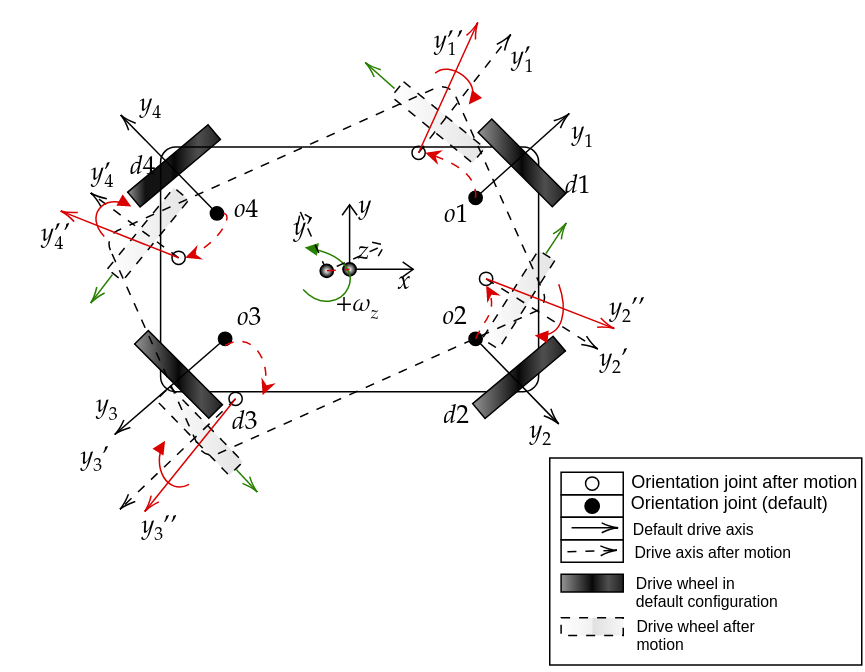
\includegraphics[scale=0.46]{images/exp1.png}
%	\end{center}
%	\caption{Experiment 1}
%	\label{fig:exp1}
%\end{figure}
%
%\paragraph{}The robot motion is interpreted based on the results obtained from the solver. The resultant motions are then compared with the actual or physical behavior of the system. By analyzing the \textit{base acceleration} values, it is observed that the robot simultaneously rotates ($\omega_z$) and accelerates backwards (negative x acceleration). This is shown in the figure \ref{fig:exp1}, with dotted lines. Additionally, the resultant \textit{joint accelerations} portray how the orientation and drive joints rotate (accelerate) given the external torque. 
%
%\subsection{Estimated motion of robot platform}
%The application of external torque causes the base to accelerate in the direction of the torque. However, the caster joints orient themselves opposite direction with respect to the base. This behavior is due to the inertia of the wheel, that introduces a delay in rotation and generates a reaction force. In the physical system, the friction at the contact point and virtual sliding and rolling constraints also contributes to this reaction force. However, the solver only models sliding constraints and do not explicitly model the friction. Therefore, as seen in the table \ref{tab:experiment}, the acceleration of orientation joints are negative. The axes ($y_1'', y_2'', y_3'', y_4''$) in the figure \ref{fig:exp1}, depicts the default wheel axis and also wheel and the axes ($y_1', y_2', y_3', y_4'$) shows the resultant drive wheel axis caused due to the rotation of orientation joints. Additionally, the magnitudes of all the joint acceleration is expected to be same. But, only two of the values are consistent. The orientation joints on right side (o2 and o3 in figure \ref{fig:exp1}) have higher acceleration that those on left-side (o1 and o4).
%
%% This inequality is due to the rectangular base. In case of a square base, all the joint accelerations would be same.
%
%\paragraph{}Although, the caster joints introduces a delay and rotates opposite direction with respect to the base, the drive wheels accelerate (rotate about \textit{y-axis}) in the same direction as robot base. Referring to the frame assignments in figure \ref{fig:tree-MPO}, the angular acceleration of drive wheels result in negative values. Additionally, the drive joints have approximately same acceleration as the base acceleration ($\omega_z$). The difference is introduced due to the caster offset and the reaction force generated at caster joints.
%
%\paragraph{}Considering the base acceleration, when a positive torque of 10 units is applied to a robot base, it is expected to have a positive angular acceleration. This reasoning do not completely apply for all system (such as a spring system). For interpreting the magnitudes, the general relation between the torque and angular acceleration is considered, which is given by,
%\begin{equation}\label{eq:t}
%	\tau = I_{zz} \dot{\omega}_z
%\end{equation}
%where, $I_{zz}$ is moment of inertia about \textit{z-axis}, which is equal to 3.68 (obtained from URDF model of the robot base). Substituting for $\tau$, results in angular acceleration $\omega_z$ of 2.71 rad/$s^2$. The deviation from the desired and actual acceleration values is 1.21. The difference is because, the equation given in \ref{eq:t}, do not consider the wheel joints. Additionally, the solver results in linear acceleration $\dot{v}_x$, which is not expected in physical behavior.  

%\section{Experiment 2}
%In this experiment, a linear force of 50 units is applied at the base. i.e., $f_x = 50$ and joint torques are 0. The figure \ref{fig:exp2} exhibits the initial and resultant configuration of the robot base due to the external force. The computed \textit{joint accelerations} and \textit{base acceleration} are interpreted for the resultant motion of the base. Since the force is applied at the base (i.e., \textit{root} of the kinematic tree structure), the resultant accelerations are computed in the final outward sweep.
%
%\begin{figure}[h!]
%	\begin{center}
%		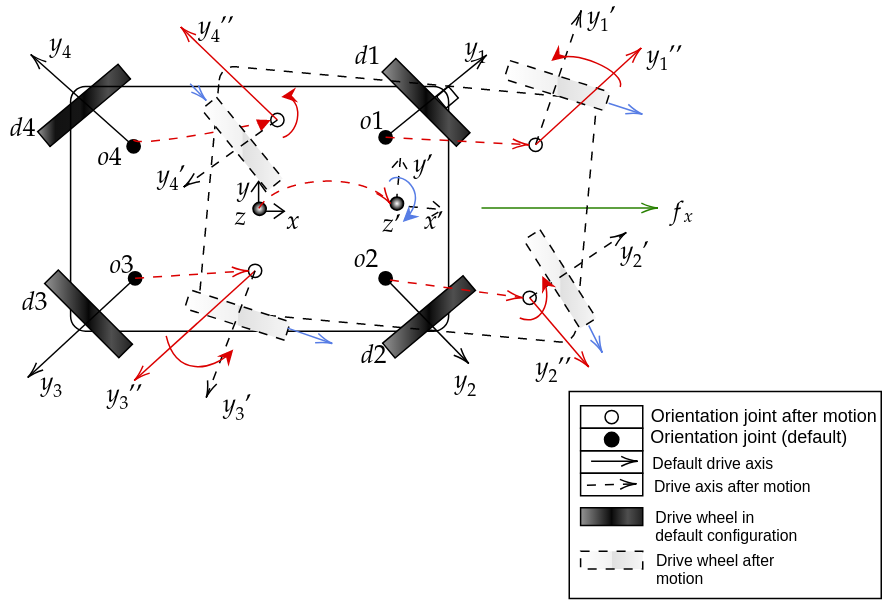
\includegraphics[scale=0.46]{images/exp2.png}
%	\end{center}
%	\caption{Experiment 2}
%	\label{fig:exp2}
%\end{figure}
%
%\paragraph{}From the \textit{base acceleration} values, it is observed that the robot simultaneously rotates ($\omega_z$) and accelerates forward (positive x acceleration). This is shown in the figure \ref{fig:exp2}, with dotted lines. Additionally, the resultant \textit{joint accelerations} portray how the orientation and drive joints rotate (accelerate) given the external force. 
%
%\subsection{Estimated motion of robot platform}
%
%When a linear force is applied at the base, the robot is expected to accelerate forward, i.e, in the direction of applied force (according to Newton's second law~\cite{newton1833philosophiae}). In a physical system, when the robot is pulled forward,  the caster joints that are initially oriented inwards, will begin rotate outwards. Because of the inertia of the drive wheel, a reaction force is generated at the drive wheel's point of contact on ground, that causes the orientation joints to rotate outwards (positive z-direction). Interpreting the results from the solver, the accelerations of orientation joints are positive and hence same as the expected behavior (in figure \ref{fig:exp2}, the joint axes ($y_1'', y_2'', y_3'', y_4''$) are initial configuration and axes ($y_1', y_2', y_3', y_4'$) are resultant configuration of joint axes due to the force). 
%
%When caster joints rotate outwards, simultaneously, the drive wheels are expected to orient roughly in the direction of force and accelerate forward (positive y-axis). Comparing this interpretation with the solver results, it is observed that the drive joint acceleration are positive. Additionally, the magnitude of drive joints is expected to be isomorphic with linear acceleration of the base. Based on this interpretation, the obtained values of drive joint accelerations and linear acceleration of base (in table \ref{tab:experiment}) are closer to each other. The error ($\sim$ 0.01) is due to caster offset and the inertia of the wheel.   
%%Furthermore, the delay introduced by the caster joints, causes the base to rotate clockwise (blue arrow at the center of the base, as shown in figure \ref{fig:exp2}).
%
%%Considering the computed joint accelerations, it is observed that the orientation joints have positive values . As mentioned in the first experiment, in a physical system, the caster joints rotate in the opposite direction, with respect to the base, due to the inertia of the wheel. Similarly, in this case, the linear force tends to rotate the caster joints in positive z direction and aligns the drive wheels linearly.
%
%%\paragraph{}Additionally, the resultant accelerations of drive joints (both direction and magnitude) must approximate to the overall acceleration of the base. It is observed from the results that the acceleration are positive (table \ref{tab:experiment}), which means that the drive wheels accelerate in the applied force direction. The magnitudes of each drive wheels are closer to $0.158$ ($\dot{v}_x$, linear acceleration of base).  
%
%
%According to Newton's second law of motion~\cite{newton1833philosophiae}, the relation between force and acceleration is given by,
%\begin{equation}\label{eq:f=ma}
%f_x = m \dot{v}_x
%\end{equation}
%Here, $m = 180kg$, mass of base (according to the technical dimension provided in MPO-700 operating manual~\cite{MPO700}). By substituting the known variables in the equation \ref{eq:f=ma}, linear acceleration $\dot{v}_x = 0.277$ m/s. The error between the calculated and obtained acceleration values (in table \ref{tab:experiment}) is 0.119. This deviation is acceptable, since the equation \ref{fig:MPO-700}, do not consider various other factors like the kinematic tree model, orientation joints, the wheel offset, etc. However, the base is not expected to have angular acceleration. Additionally, in terms of magnitude, the angular acceleration is greater than linear acceleration. This result is unacceptable in the actual behavior. 

\subsubsection*{Case 3}
\hspace{20pt}In previous cases, only external force or torque was applied at the base and the resultant wheel accelerations were analyzed. However, in this case, the drive wheels are explicitly commanded by feed-forward torques, and the behavior/motion of base is analyzed. 

When a positive torque is applied to the drive joints, it is expected to produce \textit{positive} acceleration. Due to the inertia of the base, the caster joints rotate in the opposite direction, with respect to base (\textit{positive} angular z according to right hand rule). Similarly, in the obtained results, it is observed that all the joint accelerations (caster and drive) are positive. 

At the base, it is expected to see angular acceleration in the direction of drive joints (negative z value). But the obtained result is zero. 

\subsubsection*{Case 4}
\hspace{20pt}The extended solver is also evaluated for \textit{constraint satisfaction}. As mentioned earlier, the wheels are constrained along \textit{angular-x}, \textit{linear-y} and \textit{linear-z} directions. In this case, first constraint (\textit{angular-x}) is evaluated. It is expected to have zero acceleration at joints and base. Observing the obtained results, it is verified that for the current wheel configuration the solver satisfies the given constraint.

\subsubsection*{Case 5}
\hspace{20pt}In this case, the extended solver is evaluated for \textit{linear-z} constraint. It is expected to have zero acceleration at joints and base and is reciprocated by the obtained results.

\subsubsection*{Wheel configuration 2}
The second wheel configuration for which the extended solver is evaluated, is given in table \ref{tab:experiment}. 

\subsubsection*{Case 1}
\hspace{20pt}An external torque of 10 units is applied at the base. Physically, the base is expected to rotate in the direction of applied torque (positive). As mentioned earlier, the caster joints are expected to rotate in opposite direction with respect to the base, due to the inertia of the drive wheels. Based on this interpretation, the orientation joints are expected to rotate in negative direction. But the solver results are inconsistent, where two of the caster joints (o1 and o4) are positive and other two joints (o2 and o3) are negative. Additionally, in terms of magnitude, the drive joints are expected to have higher acceleration than caster. This behavior is not reciprocated by the obtained results. 

%Nevertheless, the drive joints are expected to accelerate in the direction of base rotation. Therefore, the drive joint acceleration are expected to be negative (based on right-hand rule). 

Although, the caster joints introduces a delay and rotates opposite direction with respect to the base, the drive wheels are expected to accelerate (rotate about \textit{y-axis}) in the direction of base rotation. Referring to the frame assignments in figure \ref{fig:tree-MPO}, the angular acceleration of drive wheels result in negative values. But the solver results are positive.  

Considering the base acceleration, when a positive torque of 10 units is applied to a robot base, it is expected to have a positive angular acceleration. Considering the general relation between the torque and angular acceleration (equation \ref{eq:t}), the result is expected to be $\omega_z$ of 2.71 rad/$s^2$, which is quite far from the obtained value.

\subsubsection*{Case 2}
\hspace{20pt}In this case, a linear force of 50 units is applied at the base. i.e., $f_x = 50$ and feed-forward torques are 0. The robot is expected to accelerate forward, i.e, in the direction of applied force. It is expected to have positive acceleration in drive joints and approaximately zero acceleration at caster joints. However, the results show that both joints do not accelerate, whereas, base has linear acceleration.

Interpreting the magnitude of base acceleration by considering equation \ref{eq:f=ma},
linear acceleration $\dot{v}_x = 0.431$ m/s. The deviation is $\approx$ 0.07, and is in expected range, since the equation do not consider other factors like the kinematic tree model, orientation joints, the wheel offset, etc. 

\subsubsection*{Case 3}
\hspace{20pt}In this case, the drive wheels are explicitly commanded by feed-forward torques, and the behavior/motion of base is analyzed. 
When a positive torque is applied to the drive joints, it is expected to produce \textit{positive} linear acceleration at base, which is not observed in results (\ref{tab:experiment}). 

Analyzing the joints acceleration by considering the equation \ref{eq:t}. Here, $I_{zz}$ is 0.015 as obtained from URDF model. On substituting the values, the expected joint acceleration is 66.67 rad/$s^2$. The obtained result (65.71) is approximately the same. Since the equation $\ref{eq:t}$ do not consider the wheel joints, the deviation from the actual value is expected.

\subsubsection*{Case 4}
\hspace{20pt}In this case, the extended solver is tested for \textit{angular-x} constraint. It is expected to have zero acceleration at joints and base and obtained results are same as expected.

\subsubsection*{Case 5}
\hspace{20pt}In this case, the extended solver is tested for \textit{linear-y} constraint. It is expected to have zero acceleration at joints and base, which is not observed in results.

\subsubsection*{Case 6}
\hspace{20pt}In this case, the extended solver is tested for \textit{linear-z} constraint. It is expected to have zero acceleration at joints and base and obtained results are same as expected.

%Since, the drive joints are expected to accelerate forward, due to its configuration (45$^0$ orientation), the base rotates in negative z direction. 


%Considering the resultant base acceleration, it can be interpreted that the robot is simultaneously rotating and moving diagonally in the workspace.
%In this experiment, no external force is given, the joint torques are applied to drive wheels. In a physical system, the joint torques applied to the wheels result in acceleration of the system. The results show that the base has acceleration along linear-x, linear-y and angular-z. 

%\begin{figure}[h!]
%	\begin{center}
%		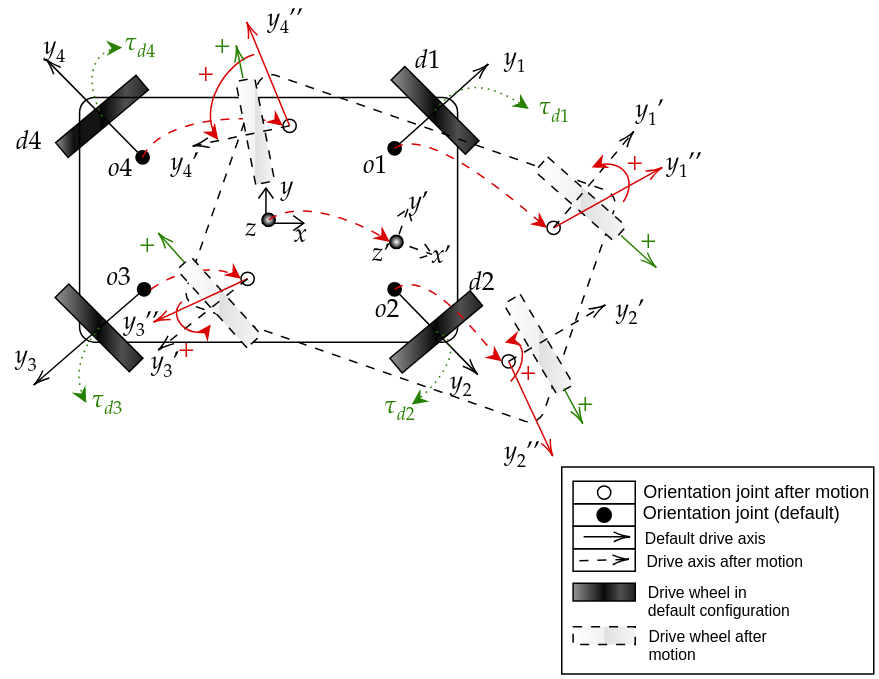
\includegraphics[scale=0.46]{images/exp3.png}
%	\end{center}
%	\caption{Experiment 3}
%	\label{fig:exp3}
%\end{figure}

\section{Task singularities}
There are certain conditions where the task might reach singularity. One of these singularity cases are explained in this section. 

\begin{figure}[h!]
	\begin{center}
		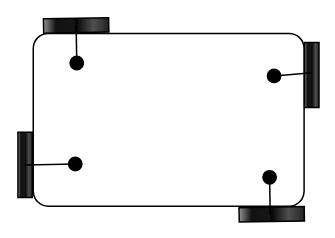
\includegraphics[scale=0.4]{images/a.png}
	\end{center}
	\caption{Wheel configuration explaining task singularity}
	\label{fig:sing}
\end{figure}

Consider a case where the wheels are configured as shown in figure \ref{fig:sing}, and when an external force is applied (either in X or Y directions), the wheel motions contradict to each other, and hence \textit{singularity} occurs. In the extended algorithm, the singularity can be detected at \textit{inertia matrix}, $H_0^A$ (equation \ref{eq:cartesian-acceleration}). The controller must explicitly command the wheels to overcome the singular configurations. 


\section{Conclusion}
The chapter presents experimental evaluation of extended solver. The obtained results are assumed to be erroneous since the interpretation of these values does not agree with the corresponding  simulated motion/behavior of the system. Two possible issues are,

\begin{enumerate}
	\item The \textit{Rigid-body inertia} specification in kinematic tree model. According to the KDL convention, the \textit{rigid-body inertia} frame is represented in \textit{tip} frame of segment. And the inertia from URDF model is represented with respect to \textit{root} frame. However, even after transforming inertial frame according to the convention, the model do not appear to provide expected results.
%	The tree structure is modeled using KDL conventions. However, the conventions followed in algorithm, KDL and URDF model differs and hence it is difficult to trace back
	\item Generally, the solver computes desired motion of the system while resolving the \textit{constraints}. When an external force or torque is applied to the system, and if it violates the constraints in any way, then the solver calculates corresponding constraint magnitudes to nullify the effect of external input. In the experiment above, the solver results are evaluated for the constraint satisfaction. It is observed that the calculated constraint magnitudes, $\nu_{float}$ (equation \ref{eq:nu-float}) is not sufficient to nullify the external force (equation \ref{eq:cartesian-acceleration}). 
\end{enumerate}  

%\begin{figure}[h!]
%	\begin{center}
%		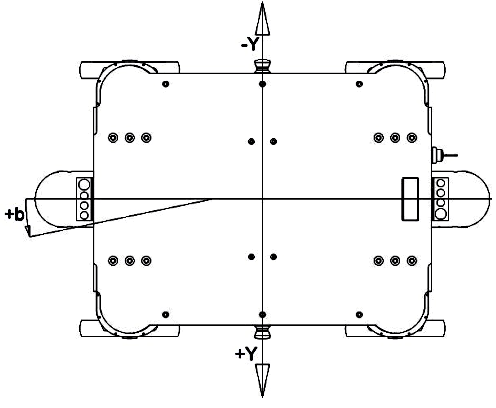
\includegraphics[scale=0.4]{images/top-view.png}
%	\end{center}
%	\caption{Experiment for analyzing constraint satisfaction}
%	\label{fig:top-view}
%\end{figure}
%
%\paragraph{}The wheels are initially configured as given in the above figure. When an external force is applied in \textit{y-direction}. The robot is not expected to move, due to the sliding constraint. However, the solver results in non-zero acceleration at the base. 






%If external force or torque applied to a system, violates these constraints, then the solver computes 
%
%The virtual or/and physical constraints of a system is modeled in the solver.   




















